\documentclass[12pt, letterpaper]{article}

\usepackage[margin=1in]{geometry}
\usepackage[spanish]{babel}
\usepackage{times}
\usepackage{float}
\usepackage{graphicx}
\usepackage{subcaption}
\usepackage[backend=biber,style=ieee]{biblatex}
\usepackage[hidelinks]{hyperref}

\setlength{\parindent}{0cm}
\setlength{\parskip}{8pt}
\graphicspath{{./img/}}
\addbibresource{biblio.bib}

\title{Docker}
\author{Carranza Ochoa, José David \\ Ríos Lira, Gamaliel}
\date{\today}

\begin{document}
\maketitle

\section{Introducción}
Actualmente, los sistemas de información se tienen que implementar bajo 
ciertas arquitecturas un tanto complejas, con la finalidad de aumentar su 
escalabilidad. Para llevar a cabo lo anterior, muchas veces se tiene que hacer 
uso de múltiples subsistemas, los cuales se despliegan de forma independiente.  
Lógicamente, es complicado que cada subsistema que se implementa, se 
despliegue en un servidor físico distinto debido al costo de los 
mismos\footnote{Y más aún cuando se habla de soluciones basadas en la nube, en 
la que muchas veces no sabemos con exactitud en qué lugar físico se están 
desplegando las aplicaciones}.

Es importante mantener cada subsistema aislado de los demás ya que cada uno de 
ellos podría tener algunos requerimientos de configuración específicos e 
incluso correr sobre diferentes sistemas operativos. Este trabajo aborda una 
investigación acerca de la herramienta \textit{Docker} con la finalidad de 
exponer sus características fundamentales y su importancia dentro de las áreas 
de tecnologías de la información actualmente. Lo anterior bajo un marco de 
referencia orientado a la materia de Sistemas Operativos.

\section{Desarrollo}
\subsection{Máquinas virtuales}
El concepto de máquina virtual (VM por sus siglas en inglés) se trata de la 
implementación de arquitecturas de hardware real a través de software. Visto 
desde otro punto de vista, se puede decir que se trata de implementar el 
comportamiento de una máquina totalmente diferente (\textit{guest}) a través 
de otra máquina (\textit{host}). Por lo general, para la administración de las 
máquinas virtuales se requiere de un programa especializado denominado 
\textit{hypervisor}.

El problema que traen consigo las máquinas virtuales es que agregan mucha 
carga de trabajo al \textit{host} debido a la capa de abstracción que requiere 
el \textit{hypervisor}. Con esto, su ejecución podría llegar a tornarse lenta.

\subsection{Contenedores}
Los contenedores son una aproximación para resolver las desventajas que traen 
consigo las máquinas virtuales. Son abstracciones en la capa de la aplicación 
que empaquetan el código y las dependencias juntas. La idea general es hacer 
paquetes de software que incluyan todos los elementos necesarios para ejecutar 
las aplicaciones en cualquier momento, pero de tal forma que al momento de la 
ejecución únicamente haya un sistema operativo en ejecución (el del 
\textit{host}).  Esto se logra haciendo que el núcleo, también concido como 
\textit{kernel}, se comparta entre todos los conenedores. Este es el principio 
de funcionamiento a través del cual funciona \textit{Docker}.

La utilización de contenedores trae consigo las siguientes ventajas:
\begin{itemize}
  \item \textbf{Separación de responsabilidades:} Los el equipo de desarrollo 
  se enfoca en la lógica y el equipo de soporte se encarga de desplegar y 
  nadie se preocupa por las configuraciones de las aplicaciones.
  \item \textbf{Portabilidad:} Los contenedores se pueden ejecutar 
  prácticamente en cualquier lugar. Desde servidores físicos, servidores en la 
    nube e incluso dentro de  máquinas virtuales.
  \item \textbf{Aislamiento:} Los contenedores virtualizan los recursos de 
  CPU, memoria, almacenamiento y red a nivel de sistema operativo (de forma 
  lógica).
\end{itemize}

Adicionalmente, una de las ventajes de los contenedores es que ocupan mucho 
menos espacio en memoria que las máquinas virtuales (las imágenes son 
típicamente de unos cuantos MB de tamaño), pueden manejar más aplicaciones y 
requieren de la utilización de menos sistemas operativos.

\subsection{Qué es Docker}
\textit{Docker} es una plataforma para desarrolladores y administradores de 
sistemas que sirve para desarrollar, desplegar y ejecutar aplicaciones con 
contenedores. De forma general, a través de \textit{Docker} y las interfaces 
que proporciona, se pueden crear, modificar, borrar e interactuar internamente 
con los contenedores de una aplicación. El uso de contenedores de Linux para 
desplegar aplicaciones es denominado contenerización (del inglés 
\textit{containerization}).  Particularmente, la utilización de contenedores 
no es algo nuevo; sin embargo, su uso para desplegar aplicaciones de forma 
sencilla sí lo es.

En la Figura \ref{fig:vm-vs-docker} se puede apreciar una comparación entre el 
funcionamiento de una máquina virtual contra el funcionamiento de 
\textit{Docker}. Es posible apreciar la gran carga de trabajo que trae consigo 
la utilización de diferentes sistemas operativos para ejecutar diferentes 
aplicaciones, lo cual evidentemente utiliza más recursos de hardware. Por otra 
parte, \textbf{Docker} únicamente utiliza un sistema operativo y a través de 
las capas de abstracción que proporciona, trabajando en conjunto con las 
funcionalidades de Linux, es posible desplegar contenedores (que únicamente 
traen consigo configuraciones a nivel de aplicación).

\begin{figure}[H]
  \centering
  \begin{subfigure}[b]{0.45\textwidth}
    \centering
    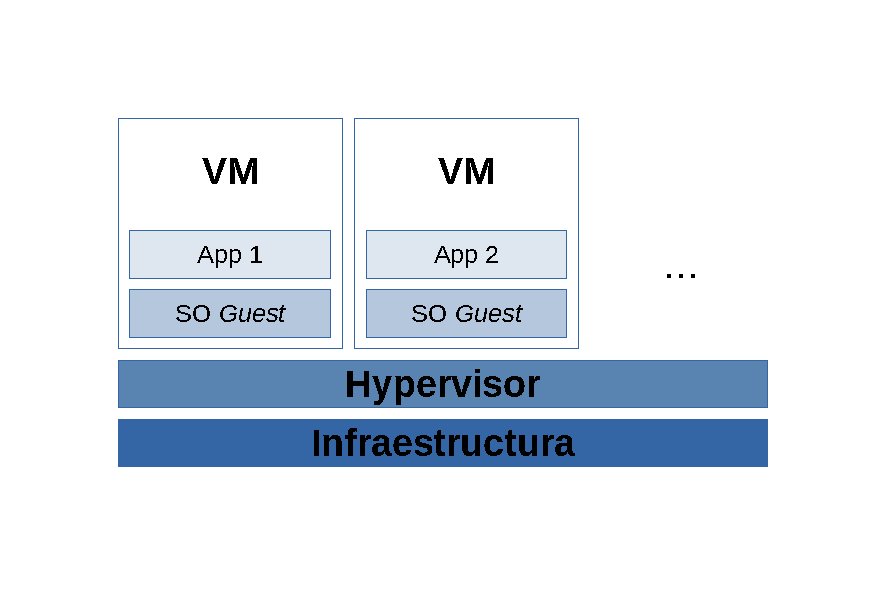
\includegraphics[width=\textwidth]{vm-schema}
    \caption{Funcionamiento de una máquina virtual}
    \label{fig:vm-schema}
  \end{subfigure}
  \begin{subfigure}[b]{0.45\textwidth}
    \centering
    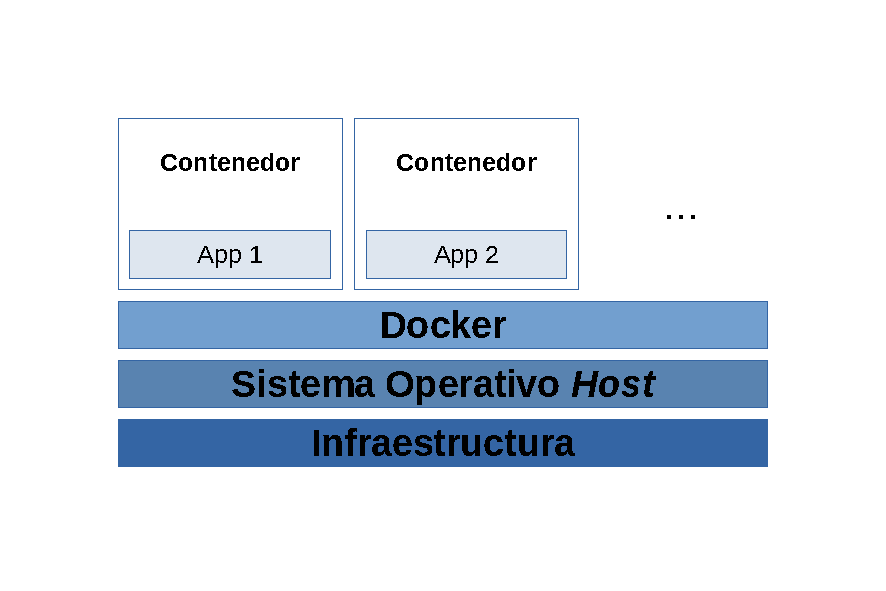
\includegraphics[width=\textwidth]{container-schema}
    \caption{Funcionamiento de contenedores Docker}
    \label{fig:container-schema}
  \end{subfigure}
  \caption{VM vs. Docker}
  \label{fig:vm-vs-docker}
\end{figure}

Además de todas las características mencionadas anteriormente acerca de los 
contenedores, los contendores de \textit{Docker} tiene las siguientes 
características específicas:
\begin{itemize}
  \item Es un \textbf{proceso} ---o grupo de procesos--- de Linux.
  \item Está \textbf{aislado} del sistema operativo \textit{host} que lo 
  aloja.
  \item Tiene una cantidad de \textbf{recursos limitada}.
  \item Cuenta con un \textbf{sistema de archivos independiente} del sistema 
  operativo \textit{host}.
\end{itemize}

Para lograr que cada uno de los contenedores tenga las características 
descritas anteriormente, \textit{Docker} necesita hacer uso de algunas 
funciones del kernel de Linux, como los \textbf{grupos de control} y los 
\textbf{namespaces}.

\subsubsection{Espacios de Nombres (namespaces)}
Tal como se sabe, una de las mayores características que debe proporcionar un 
sistema operativo es el \textbf{aislamiento}. Para el ámbito en cuestión, este 
concepto hace referencia a que los procesos en ejecución no deben preocuparse 
por los demás procesos que también están siendo ejecutados. El sistema debe 
funcionar ---idealmente--- como si fuera el único proceso en ejecución.

Con la finalidad de lograr este cometido, \textit{Docker} está diseñado de tal 
forma que hace uso de los \textit{namespaces} del kernel. La idea de los 
\textit{namespaces} es envolver los recursos globales del sistema en una 
abstracción que haga parecer que los procesos del mismo \textit{namespace} 
tienen su propia instancia de dicho recurso global. De esta forma, se obtiene 
un aislamiento entre procesos.  La idea principal de \textit{Docker} reside 
justo en este punto, ya que a través de los \textit{namespaces} se logra crear 
los contenedores como ``subsistemas'' aislados de todos los demás procesos que 
ejecuta el sistema operativo. Cuando se ejecuta un contenedor, \textit{Docker} 
crea un conjunto de namespaces para ese contenedor en específico.

Algunos de los \textit{namespaces} de Linux que \textit{Docker} utiliza 
internamente son los siguientes:
\begin{itemize}
  \item \textbf{PID.} Permite que los procesos que se encuentran en diferentes 
    \textit{PID namespaces} puedan tener el mismo identificador de proceso 
    (PID).
  \item \textbf{NET.} Permite el aislamiento de recursos relacionados con 
    redes: números de puerto, dispositivos de red, reglas de 
    \textit{firewall}, etc.
  \item \textbf{MNT.} Permite el aislamiento de unidades montadas para 
    procesos en cada instancia del \textit{namespace}. Cada proceso de una 
    instancia verá distintas jerarquías de directorios.
  \item \textbf{UTS.} Provee aislamiento de dos identificadores del sistema: 
    el \textit{hostname} y el nombre de dominio NIS.
\end{itemize}

\subsubsection{Grupos de Control (cgroups)}
Sumado a lo anterior ---y tal como ya se mencionó anteriormente---, 
\textit{Docker} también hace uso de los \textbf{grupos de control} 
(\textit{cgroups}) del kernel.  Estos le permiten compartir recursos de 
hardware disponibles con los contenedores, aplicando límites y restricciones.  
De forma breve, los \textit{cgroups} son un mecanismo para controlar los 
recursos del sistema. Cuando un \textit{cgroup} está activo, puede controlar 
la cantidad de CPU, RAM, tiempo u otros recursos que un proceso pueda 
requerir.

De forma interna, algunos de los grupos de control que \textit{Docker} utiliza 
son:
\begin{itemize}
  \item \textbf{Memory cgroup.} Limita el uso de memoria para procesos y 
    genera reportes de los recursos de memoria utilizados por cada proceso.
  \item \textbf{CPU cgroup.} Límites de utilización de la CPU para un proceso.  
    Evita que un proceso consuma mucho tiempo de CPU, evitando que esto afecte 
    negativamente al desempeño del sistema.
  \item \textbf{Devices cgroup.} Permite o restringe el acceso a dispositivos 
    par aun proceso.
\end{itemize}

\subsubsection{Sistema de archivos}
Cada contenedor, como ya se explicó anteriormente, necesita tener un sistema 
de archivos aislado que aparente ser ``único'' para el proceso que esté 
ejecutando. Esto no significa que sea totalmente independiente del sistema 
operativo \textit{host}; más bien, hace referencia a que el proceso supondrá 
que el sistema de archivos al que tiene acceso es el único disponible y no 
sabrá que internamente no es más que una sección del sistema de archivos del 
sistema \textit{host}, al cual evidentemente no tendrá acceso ---al menos no 
directamente. Esta tarea se lleva a cabo a través de una herramienta 
disponible para los sistemas operativos basados en Unix ---tal como el caso de 
Linux--- llamada \textit{chroot}. Esta herramienta hace posible invocar un 
proceso, cambiando para este y sus hijos el directorio raíz del sistema. Esto 
no es más que otra forma de aislamiento que se agrega al proceso en ejecución 
por el contenedor.

\subsection{Desventajas}
Durante la investigación elaborada, se encontró un dato muy importante de 
destacar acerca de la forma en la que trabaja \textit{Docker}. Aún cuando se 
trata de una herramienta sumamente madura y ampliamente aceptada en la 
industria ---ya que por mucho tiempo tuvo soporte de \textit{RedHat}---, su 
implementación cuenta con un detalle que los expertos en el ámbito de la 
seguridad informática siempre han criticado. La ejecución del \textit{Docker 
Deamon} ---una de las herramientas que trae integrada internamente--- necesita 
tener privilegios de \textit{root}. Con esto, la posibilidad de que un 
contenedor se libere de su ``contexto aislado'' y ejecute código en el sistema 
\textit{host} siempre está presente. Esto no es un detalle menor y aún con el 
paso del tiempo nunca ha podido ser corregido.

Lo anterior ha orillado a la creación de nuevas plataformas similares a 
\textit{Docker}. Tal es el caso del proyecto \textit{Podman}, en donde se está 
desarrollando una alternativa sumamente similar y compatible con 
\textit{Docker}, en la cual se corrige de forma definitiva el detalle antes 
mencionado.

Finalmente, la herramienta \textit{DockerHub}, un complemento de 
\textit{Docker} a través de donde se obtienen imágenes de contenedores, ha 
sido vulnerada a través de la publicación de imágenes maliciosas que algunas 
veces ejecutan procesos por detrás con la finalidad de obtener beneficios. No 
pasa esto con todas las imágenes, la mayor parte de este problema se concentra 
en imágenes \textbf{no oficiales}, publicadas por personas aisladas que no 
pertenecen a algún tipo de organización. Aún cuando esto es una desventaja, se 
puede contrarrestar haciendo uso de imágenes \textbf{oficiales}.

\section{Conclusiones}
Tal como se expuso anteriormente, \textit{Docker} es una herramienta que hace 
uso de una solución innovadora para para la gestión de contenedores. La parte 
interna de su funcionamiento está arraigada complemente a la forma en la que 
trabaja el kernel del sistema operativo, más específicamente el kernel de 
Linux ---\textit{namespaces}, \textit{cgroups}, procesos, etc. El tema resulta 
ser de amplia importancia para la materia de Sistemas Operativos, más aún 
cuando son patrones de soluciones que se utilizan actualmente en la industria.  
A pesar de esto, no todo es perfecto y en el caso de \textit{Docker}, tiene 
algunas limitantes que no son menores. Nos parece que \textit{Docker} marcó un 
antes y un despues en los aspectos relacionados con el uso de contenedores 
para desplegar aplicaciones, a tal punto que está siendo la referencia de 
partida para tecnologías emergentes.

% Impresión de Bibliografía
\clearpage
\nocite{*}
\section{Bibliografía}
\printbibliography[heading=none]

\end{document}

